\chapter{Continuous Integration}
\label{chap:continuous-integration}

The final phase of our project was to implement a CI process for Synote. Only by deploying a new version of Synote and testing it can we be sure that a feature implementation is stable and functioning. However, a Synote experiment deployment has quite a few steps (\textbf{Figure \ref{fig:synote-ci-proc}}), which can take 15-20 minutes to complete. In fact, it is completely infeasible to regularly repeat all the steps without hampering a developer's work. Since making a deployment takes  considerable time, yet continuous automated testing on remote deployments is incredibly useful, we extended our project scope to implement Synote's first CI process.

\section{Synote CI}
\label{sec:synote-ci}

A complete Synote CI process will deploy and test on the experiment deployment, followed by staging and finally production. Each stage will follow similar steps as shown in the Experiment Deployment (Step 2 of \textbf{Figure \ref{fig:synote-ci-proc}}).\\

We focused on CI for the experiment deployment since we had access to it. In this chapter, we will elucidate the key steps necessary to configure a complete CI environment using \textit{Jenkins}.\\

The key issues in this phase were:

\begin{itemize}

  \item Installing and configuring \textit{Jenkins} with SSL, restricting user access etc. (\textbf{Section \ref{subsec:setting-up-jenkins}})

  \item Synote is deployed as the user \texttt{ubuntu}, however, \textit{Jenkins} runs the build scripts as user \texttt{jenkins}. So, permissions for the deployment folders need to be rectified (\textbf{Listing \ref{lst:deployment-folder-permissions}})

  \item \texttt{jenkins} needs to have access to the \textit{PM2} (a process manager) processes started by \texttt{ubuntu} (\textbf{Listing \ref{lst:jenkins-pm2-configuration}})

  \item Running the E2E tests on a browser using a virtual display (\textbf{Section \ref{subsec:e2e-testing-on-remote}})

\end{itemize}

\begin{figure}[!hbt]
  	\centering
 	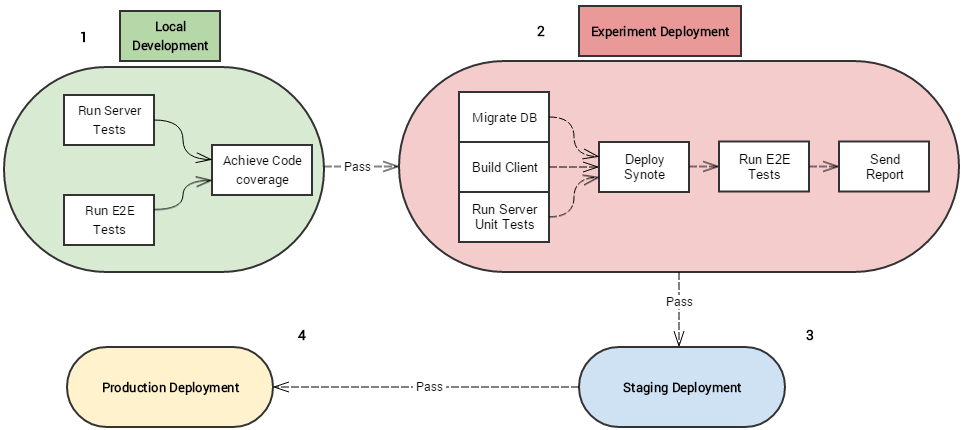
\includegraphics[width=\textwidth]{synote-ci.png}
  	\caption{Synote Continuous Integration Procedure}
 	\label{fig:synote-ci-proc}
\end{figure}

\subsection{Setting up Jenkins}
\label{subsec:setting-up-jenkins}

We began by installing \textit{Jenkins} on the experiment server (\textbf{Listing \ref{lst:install-jenkins}}). After monitoring the processes, we asked the client to upgrade the server to have 4GB RAM.\\

\begin{listing}[H]
\begin{minted}[xleftmargin=\parindent, linenos, breaklines, breakanywhere, bgcolor=lightgray, fontsize=\small]{bash}

# install Jenkins on Ubuntu (Synote Experiment Deployment)
wget -q -O - https://pkg.jenkins.io/debian/jenkins-ci.org.key | sudo apt-key add -
sudo sh -c 'echo deb http://pkg.jenkins.io/debian-stable binary/ > /etc/apt/sources.list.d/jenkins.list'
sudo apt-get update
sudo apt-get install jenkins

\end{minted}
\captionof{listing}{Install Jenkins}
\label{lst:install-jenkins}
\end{listing}

Then we added one admin account with complete \textit{Jenkins} control, and one developer account with reduced control (e.g. cannot delete projects). Finally, we needed to run \textit{Jenkins} behind a reverse proxy server (Nginx) so that SSL encryption works properly and the domain reaches it (\textbf{Listing \ref{lst:make-jenkins-available}}). The Synote experiment CI project can be seen in \textbf{Figure \ref{fig:synote-jenkins-server}}\\

\begin{listing}[H]
\begin{minted}[xleftmargin=\parindent, linenos, breaklines, breakanywhere, bgcolor=lightgray, fontsize=\small]{bash}

# nginx reverse proxy configuration for Jenkins

echo "upstream jenkins {
  server 127.0.0.1:8080 fail_timeout=0;
}

server {
  listen 80;
  server_name jenkins-cicd.synote.com; # dns for Synote CI
  return 301 https://$host$request_uri;
}

# ssl redirection

server {
  listen 443 ssl;
  server_name <synote_jenkins_ci_domain_name>;

  ssl_certificate <synote_ssl_certificate_location>;
  ssl_certificate_key <synote_ssl_private_key_location>;

  location / {
    proxy_set_header        Host $host:$server_port;
    proxy_set_header        X-Real-IP $remote_addr;
    proxy_set_header        X-Forwarded-For $proxy_add_x_forwarded_for;
    proxy_set_header        X-Forwarded-Proto $scheme;
    proxy_redirect http:// https://;
    proxy_pass              http://jenkins;
  }
}" > /etc/nginx/sites-available/jenkins

sudo service nginx restart

\end{minted}
\captionof{listing}{Make Jenkins Server Available on Nginx}
\label{lst:make-jenkins-available}
\end{listing}

\begin{figure}[!hbt]
  	\centering
 	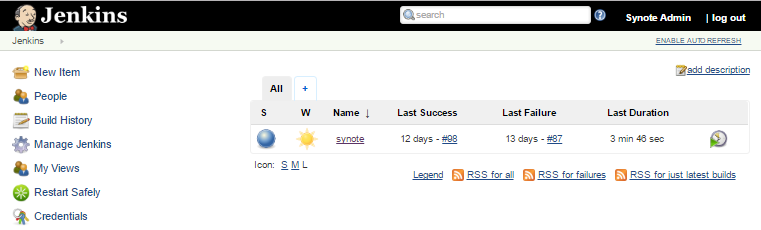
\includegraphics[width=0.78\textwidth]{jenkins.png}
  	\caption{Slack Jenkins Server}
 	\label{fig:synote-jenkins-server}
\end{figure}

\subsection{Triggering Builds}
\label{subsec:triggering-builds}

\subsubsection{Automatically}
\label{subsubsec:triggering-builds-automatically}

Builds can be triggered automatically when changes are made to the repository. In order to set this up, the following steps must be followed:

\begin{itemize}
\item Install the \textit{BitBucket Jenkins Plugin}. This plugin can be found in the \textit{Manage Jenkins} $\rightarrow$ \textit{Manage Plugins} section.

\item Once installed, go to the \textit{Jenkins} project and click \textit{Configure}. Under \textit{Build Triggers}, select the \textit{BitBucket} option (\textbf{Figure \ref{fig:bitbucket-build-trigger}}).\\

\begin{figure}[!hbt]
  	\centering
 	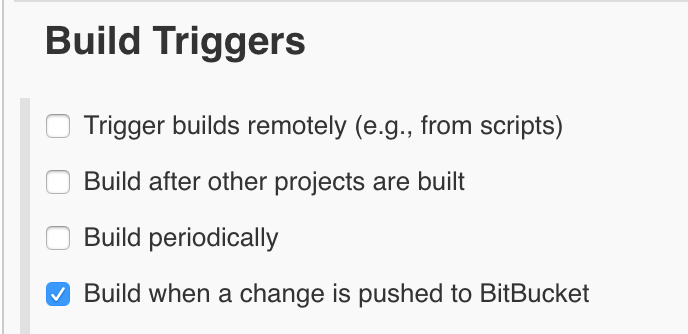
\includegraphics[width=0.5\textwidth]{bitbucket-build-trigger.png}
  	\caption{BitBucket Build Trigger}
 	\label{fig:bitbucket-build-trigger}
\end{figure}

\item Set up the \textit{BitBucket WebHook}. Go to the \textit{BitBucket} repository website under the \textit{Settings} $\rightarrow$ \textit{WebHooks} section. Click on \textit{Add webhook}, give it a name and paste in the webhook which is of the form \textit{jenkins-address:8080/bitbucket-hook/}. The current setup has this URL in place: \textit{https://jenkins-cicd.synote.com/bitbucket-hook/}. The trailing slash must be kept in the URL.\\

\begin{figure}[!hbt]
  	\centering
 	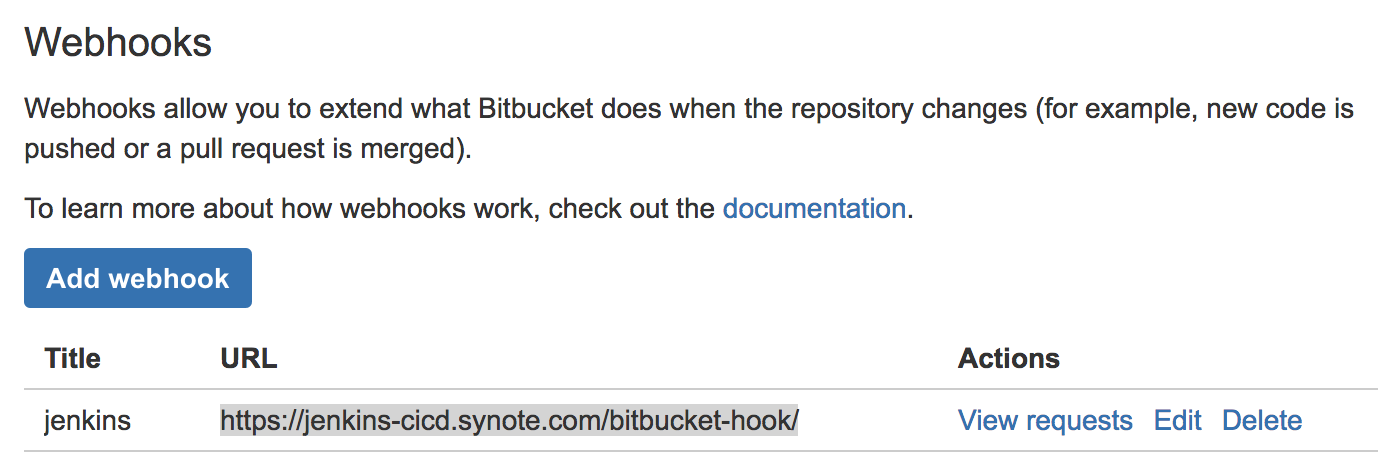
\includegraphics[width=0.78\textwidth]{bitbucket-webhook.png}
  	\caption{BitBucket WebHook}
 	\label{fig:bitbucket-webhook}
\end{figure}

\end{itemize}

\begin{figure}[!hbt]
  	\centering
 	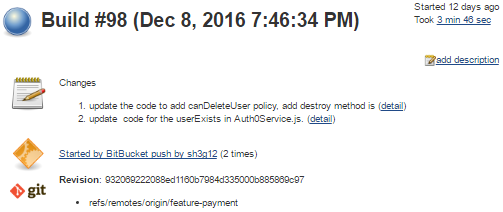
\includegraphics[width=0.78\textwidth]{jenkins-build-trigger.png}
  	\caption{Jenkins Build Trigger}
 	\label{fig:jenkin-build-trigger}
\end{figure}

\subsubsection{Manually}
\label{subsubsec:triggering-builds-manually}

Triggering a build manually is very easy. Just select a \textit{Jenkins} project and click \textit{Build Now}.

\vspace{0.5cm}

\begin{figure}[!hbt]
  	\centering
 	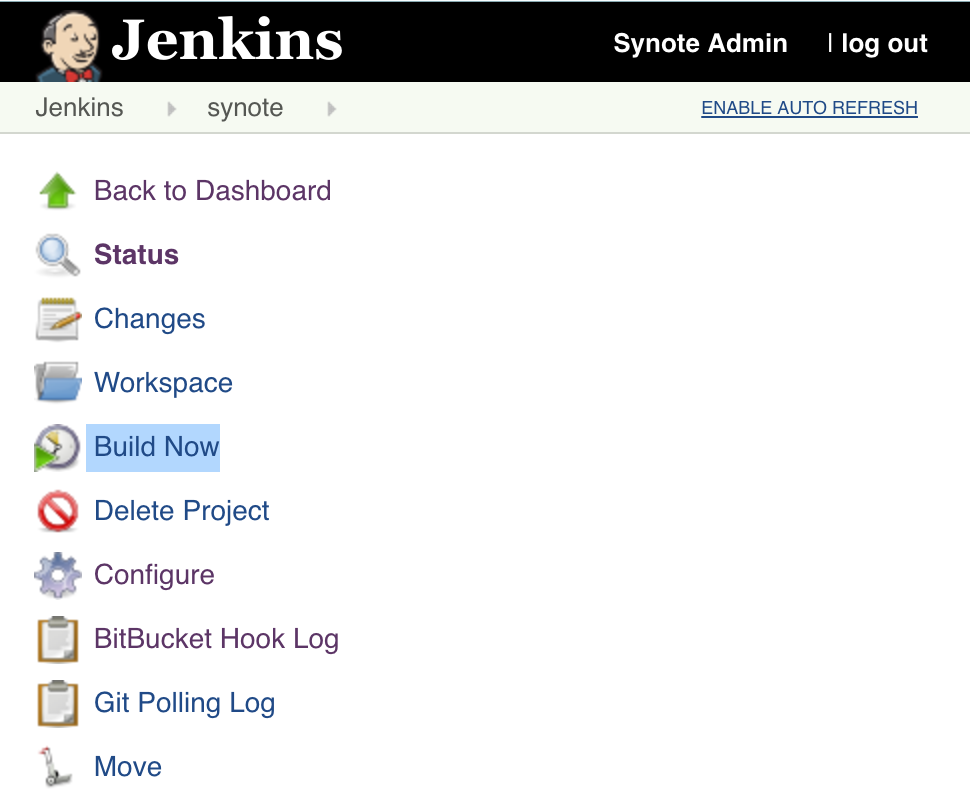
\includegraphics[width=0.6\textwidth]{triggering-builds-manually.png}
  	\caption{Triggering Builds Manually}
 	\label{fig:triggering-builds-manually}
\end{figure}

\vspace{-0.5cm}

\section{Pre-build Preparation}
\label{sec:pre-build-preparation}

We first needed to give the ownership of \texttt{npm} modules to \texttt{ubuntu} (\textbf{Listing \ref{lst:npm-permission}}), so that we could install \texttt{bower}, which is needed to resolve the client app dependencies.\\

\begin{listing}[H]
\begin{minted}[xleftmargin=\parindent, linenos, breaklines, breakanywhere, bgcolor=lightgray, fontsize=\small]{bash}

# give permission to install global npm dependecies
sudo chown -R $USER:$GROUP ~/.npm
sudo chown -R $USER:$GROUP ~/.config

\end{minted}
\captionof{listing}{Global npm Dependency Permission}
\label{lst:npm-permission}
\end{listing}

\textbf{Listing \ref{lst:jenkins-build-script-variables}} shows the different source-code locations on the experiment deployment that are concerned with the CI script. These will be necessary in the subsequent listings.\\

\begin{listing}[H]
\begin{minted}[xleftmargin=\parindent, linenos, breaklines, breakanywhere, bgcolor=lightgray, fontsize=\small]{bash}

# the repos
SYNOTE_MAIN=/home/ubuntu/synote
SYNOTE_JENKINS=$WORKSPACE
E2E_JENKINS=$WORKSPACE/../gdp8-synote-e2e-testing
E2E_MAIN=/home/ubuntu/gdp8-synote-e2e-testing
REPORTS_WEBSITE_MAIN=$E2E_MAIN/reportsWebsite

\end{minted}
\captionof{listing}{Variables Used During the Jenkins Build Script}
\label{lst:jenkins-build-script-variables}
\end{listing}

Next we give the permissions for the E2E testing and Synote deployment repo to a group that contains both \texttt{ubuntu} and \texttt{jenkins} (\textbf{Listing \ref{lst:deployment-folder-permissions}}), allowing \texttt{jenkins} to make new deployments of Synote.\\

\begin{listing}[H]
\begin{minted}[xleftmargin=\parindent, linenos, breaklines, breakanywhere, bgcolor=lightgray, fontsize=\small]{bash}

# create user group synote
sudo groupadd synote
sudo usermod -a -G synote jenkins
sudo usermod -a -G synote ubuntu

# permissions for e2e testing
sudo chown -R ubuntu: $E2E_MAIN
sudo chgrp -R synote $E2E_MAIN
sudo chmod -R 777 $E2E_MAIN

# permissions for synote
sudo chown -R ubuntu: $SYNOTE_MAIN
sudo chgrp -R synote $SYNOTE_MAIN
sudo chmod -R 777 $SYNOTE_MAIN

\end{minted}
\captionof{listing}{Deployment Folder Permissions}
\label{lst:deployment-folder-permissions}
\end{listing}

One issue was that \texttt{git} would regularly create some files that are owned by \texttt{ubuntu} and the files built by \texttt{jenkins} could not replace those. So, we remove the \texttt{.git} folders (\textbf{Listing \ref{lst:deleting-git-folders}}), since \texttt{jenkins} will replace them with more recent versions.\\

\begin{listing}[H]
\begin{minted}[xleftmargin=\parindent, linenos, breaklines, breakanywhere, bgcolor=lightgray, fontsize=\small]{bash}

# delete the .git folders from both repos
# since it creates files for ubuntu account only
rm -rf $SYNOTE_MAIN/.git
rm -rf $E2E_MAIN/.git

\end{minted}
\captionof{listing}{Deleting .git Folders}
\label{lst:deleting-git-folders}
\end{listing}

Finally, we need to give \texttt{jenkins} access to the deployment processes created by \texttt{ubuntu} so that it could restart them (\textbf{Listing \ref{lst:jenkins-pm2-configuration}}).\\

\begin{listing}[H]
\begin{minted}[xleftmargin=\parindent, linenos, breaklines, breakanywhere, bgcolor=lightgray, fontsize=\small]{bash}

# Make locally installed programs available to jenkins
export PATH=${PATH}:/home/ubuntu/.nvm/v4.3.2/bin
export PM2_HOME="/home/ubuntu/.pm2"

# Make pm2 tasks started by 'ubuntu' available to 'jenkins'
sudo chmod 777 /home/ubuntu/.pm2/pub.sock
sudo chmod 777 /home/ubuntu/.pm2/rpc.sock

\end{minted}
\captionof{listing}{PM2 Configuration for Jenkins}
\label{lst:jenkins-pm2-configuration}
\end{listing}

\section{Synote Build}
\label{sec:synote-build}

Once a build is triggered, \textit{Jenkins} pulls the latest Synote repository. Then \texttt{jenkins} builds the server (\textbf{Listing \ref{lst:building-synote-server}}), the client (\textbf{Listing \ref{lst:building-synote-client}}) and moves the static assets to \texttt{backend/}. Finally, the complete build folder replaces \texttt{ubuntu}'s Synote deployment folder (\textbf{Listing \ref{lst:replace current deployment source}}).\\

\begin{listing}[H]
\begin{minted}[xleftmargin=\parindent, linenos, breaklines, breakanywhere, bgcolor=lightgray, fontsize=\small]{bash}

# building the server
cd $SYNOTE_JENKINS/backend
npm install

\end{minted}
\captionof{listing}{Building Synote Server}
\label{lst:building-synote-server}
\end{listing}

\begin{listing}[H]
\begin{minted}[xleftmargin=\parindent, linenos, breaklines, breakanywhere, bgcolor=lightgray, fontsize=\small]{bash}

# building the client
cd $SYNOTE_JENKINS/frontend
npm install
bower install
grunt build:experiment

\end{minted}
\captionof{listing}{Building Synote Client}
\label{lst:building-synote-client}
\end{listing}

\begin{listing}[H]
\begin{minted}[xleftmargin=\parindent, linenos, breaklines, breakanywhere, bgcolor=lightgray, fontsize=\small]{bash}

# replace the assets in /backend with the new frontend build
cp -RT $SYNOTE_JENKINS/frontend/dist/ $SYNOTE_JENKINS/backend/assets/

# Copy the synote repo from 'jenkins' to synote in 'ubuntu'
cp -RT $SYNOTE_JENKINS $SYNOTE_MAIN

\end{minted}
\captionof{listing}{Replace the Current Experiment Deployment Source}
\label{lst:replace current deployment source}
\end{listing}

\subsection{Automated Database Migration}
\label{subsec:automated-database-migration}

When a change is made in the schema, databases from various sites will need to be updated at some point. This is done via a SQL migration script. Problems may arise whenever changes from the migration are already present on the database that we are running the script against. This stops the script execution making it cumbersome to automate.

\begin{listing}[H]
\begin{minted}[xleftmargin=\parindent, linenos, breaklines, breakanywhere, bgcolor=lightgray, fontsize=\small]{bash}

# Run database migration
# Currently it's hardcoded to the latest migration but in the future,
# this should be decided on runtime depending on the database version
cd $SYNOTE/backend/db/migrate
mysql -u synote '-p<mysqlpass>' synote_server_experiment < procedures.sql # update procedures
mysql -u synote '-p<mysqlpass>' synote_server_experiment < v0.9.0-v0.10.0.sql # do migration

\end{minted}
\captionof{listing}{Automated DB Migration}
\label{lst:automated-db-migration}
\end{listing}

\subsubsection{SQL Procedures}
\label{subsubsec:sql-procedures}

To overcome the above issue, we can use \textit{MySQL} procedures. These are in essence functions to which we can add useful logic. In our case, we wish to check if a change is already present and if it is, we ignore the error so the migration script can carry on unhindered. An example procedure can seen in \textbf{Listing \ref{lst:sql-procedure}}.

\begin{listing}[H]
\begin{minted}[xleftmargin=\parindent, linenos, breaklines, breakanywhere, bgcolor=lightgray, fontsize=\small]{sql}
DROP PROCEDURE IF EXISTS addColumnSafe;
DELIMITER //
CREATE PROCEDURE addColumnSafe
  (IN _table VARCHAR(64),IN _column VARCHAR(64),IN _type varchar(64))
BEGIN
  DECLARE _stmt VARCHAR(1024);
  SET @ddl = CONCAT
    ('ALTER TABLE ', _table, ' ADD COLUMN ', _column, ' ', _type);
  IF NOT EXISTS
  (
    SELECT * FROM information_schema.COLUMNS
    WHERE TABLE_NAME=_table AND COLUMN_NAME=_column
  )
  THEN
    PREPARE _stmt FROM @ddl;
    EXECUTE _stmt;
    DEALLOCATE PREPARE _stmt;
  END IF;
END //
DELIMITER ;
\end{minted}
\captionof{listing}{SQL Procedure}
\label{lst:sql-procedure}
\end{listing}

\pagebreak

Before doing any migration, the procedures must be updated:

\begin{listing}[H]
\begin{minted}[xleftmargin=\parindent, linenos, breaklines, breakanywhere, bgcolor=lightgray, fontsize=\small]{bash}

mysql -u some_user -p some_database < ~/backend/db/migrate/procedures.sql

\end{minted}
\captionof{listing}{Updating SQL Procedures}
\label{lst:updating-sql-procedures}
\end{listing}

\subsubsection{Automated Migration Convetion}
\label{subsubsec:automated-migration-convention}

Whenever changes are needed in the schema, a procedure must be used to avoid the duplicate change error. There should be a procedure for all schema alterations (new table, new table column, etc). Within the migration script, the procedure is called with the required parameters.

\begin{listing}[H]
\begin{minted}[xleftmargin=\parindent, linenos, breaklines, breakanywhere, bgcolor=lightgray, fontsize=\small]{sql}

CALL addColumnSafe('some_table', 'some_column', 'some_type')

\end{minted}
\captionof{listing}{Calling an SQL Procedure}
\label{lst:calling-an-sql-procedure}
\end{listing}

If we try to insert data that is already present, \textit{MySQL} will complain and cease execution. To avoid this, we append this line after every data insertion statement:

\begin{listing}[H]
\begin{minted}[xleftmargin=\parindent, linenos, breaklines, breakanywhere, bgcolor=lightgray, fontsize=\small]{sql}

ON DUPLICATE KEY UPDATE id=id;

\end{minted}
\captionof{listing}{Avoiding Duplicate Data Insertion Errors}
\label{lst:avoiding-duplicate-data-insertion-errors}
\end{listing}

This works under the assumption that each table has a primary key called \texttt{id} which is true with the currently used ORM.
\\

Details on how database migration is handled can be found in \texttt{CONTRIBUTING.md} in the Synote repository.

\subsection{Restarting the New Build}
\label{subsec:restarting-the-new-build}

PM2 is a process manager that keeps processes alive even when users log off. Synote experiment deployment is kept alive as a PM2 process, which is restarted by \texttt{jenkins} at this stage (\textbf{Listing \ref{lst:restart-experiment-deployment}}).\\

\begin{listing}[H]
\begin{minted}[xleftmargin=\parindent, linenos, breaklines, breakanywhere, bgcolor=lightgray, fontsize=\small]{bash}

# always use pm2 app name to restart
pm2 restart synote_experiment

\end{minted}
\captionof{listing}{Restart Experiment Deployment}
\label{lst:restart-experiment-deployment}
\end{listing}

\section{E2E Testing on Remote}
\label{subsec:e2e-testing-on-remote}

To run the E2E tests, we first need the latest E2E test suite (located on a different repository) and prepare it for use (\textbf{Listing \ref{lst:configure-latest-e2e-testing-repo}}) in a similar process to Synote deployment (described in \textbf{Section \ref{sec:synote-build}}).\\

\begin{listing}[H]
\begin{minted}[xleftmargin=\parindent, linenos, breaklines, breakanywhere, bgcolor=lightgray, fontsize=\small]{bash}

# cloning e2e repo
rm -rf $E2E_JENKINS

cd $SYNOTE_JENKINS/..
git clone git@bitbucket.org:sh3g12/gdp8-synote-e2e-testing.git

# copy over the content to 'ubuntu' e2e testing from 'jenkins'
cp -RT $E2E_JENKINS $E2E_MAIN

# install e2e main dependencies
cd $E2E_MAIN
npm install

\end{minted}
\captionof{listing}{Configure the Latest E2E Testing Repository}
\label{lst:configure-latest-e2e-testing-repo}
\end{listing}

Synote's E2E test HTML reports are made available through a simple website (which is deployed by Nginx in a similar process to \textbf{Listing \ref{lst:make-jenkins-available}}). This website is packaged with the E2E tests. So, we must redeploy for the latest reporting website (\textbf{Listing \ref{lst:deploy-latest-reporting-website}}).\\

\begin{listing}[H]
\begin{minted}[xleftmargin=\parindent, linenos, breaklines, breakanywhere, bgcolor=lightgray, fontsize=\small]{bash}

# install reports website dependencies
cd $REPORTS_WEBSITE_MAIN
npm install

# restart the reporting server
pm2 restart reports_website

\end{minted}
\captionof{listing}{Deploy Latest Reporting Website}
\label{lst:deploy-latest-reporting-website}
\end{listing}

E2E tests run in a browser which requires a display. So, a virtual display (Xvfb) is installed, along with the helper libraries and finally the browsers themselves (\textbf{Listing \ref{lst:xvfb-browser-install}}).\\

\begin{listing}[H]
\begin{minted}[xleftmargin=\parindent, linenos, breaklines, breakanywhere, bgcolor=lightgray, fontsize=\small]{bash}

# install virtual display library
sudo apt-get install xvfb

# install Packages Required by browsers
sudo apt-get install x11-xkb-utils xfonts-100dpi xfonts-75dpi
sudo apt-get install xfonts-scalable xserver-xorg-core
sudo apt-get install dbus-x11

# install Browser
sudo apt-get install chromium-browser

\end{minted}
\captionof{listing}{Install Virtual Display Library and Browsers}
\label{lst:xvfb-browser-install}
\end{listing}

Now the installed display server and a \textit{Selenium} server are started as PM2 daemon processes  (\textbf{Listing \ref{lst:webdriver-pm2}}), so that these steps need not be performed in the future.\\

\begin{listing}[H]
\begin{minted}[xleftmargin=\parindent, linenos, breaklines, breakanywhere, bgcolor=lightgray, fontsize=\small]{bash}

# start the virtual display
echo "Xvfb :99" > $SYNOTE_JENKINS/xvfb_display.sh
pm2 start $SYNOTE_JENKINS/xvfb_display.sh

# start webdriver on the virtual display
echo "export DISPLAY=:99 && npm run start-manager" > $SYNOTE_JENKINS/depl.sh
pm2 start $SYNOTE_JENKINS/depl.sh

\end{minted}
\captionof{listing}{Start Virtual Display and Webdriver as PM2 Processes}
\label{lst:webdriver-pm2}
\end{listing}

Finally we run the tests and send the latest report link to a \textit{Slack} channel (\textbf{Listing \ref{lst:run-e2e-tests}} and \textbf{Figure \ref{fig:slack-report-link}}).\\

\begin{listing}[H]
\begin{minted}[xleftmargin=\parindent, linenos, breaklines, breakanywhere, bgcolor=lightgray, fontsize=\small]{bash}

# start testing
cd $E2E_MAIN
npm test

LATEST_HTML_REPORT="https://reports-cicd.synote.com/"`find /home/ubuntu/gdp8-synote-e2e-testing/reports/ -type f -name \*.html -printf '%T@ %p\n' | sort -n | tail -1 | cut -d'/' -f 6-`

curl -X POST -H 'Content-type: application/json' --data '{"text": "'"$LATEST_HTML_REPORT"'", "channel": "#testing", "username": "Jenkins Test Bot"}' https://hooks.slack.com/services/<webhooktoken>

\end{minted}
\captionof{listing}{Run E2E Tests}
\label{lst:run-e2e-tests}
\end{listing}

\begin{figure}[!hbt]
  	\centering
 	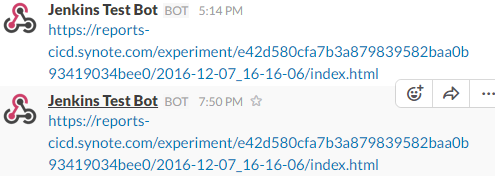
\includegraphics[width=0.78\textwidth]{slack-report-link.png}
  	\caption{Slack Report Link}
 	\label{fig:slack-report-link}
\end{figure}

\vspace{1cm}

\section{Usefulness of Synote CI}
\label{sec:usefulness-of-synote-ci}

We have found that Synote's CI allowed us to:

\begin{itemize}

  \item Write code confidently, since we can very easily run the complete deployment and be assured of regression testing.

  \item Have a record of \textit{all} the previous builds and test reports. So, we could easily track when a feature was functional or what broke a build etc. This also streamlined debugging deployment issues.

  \item Run a build without logging into the remote server itself, making deployment accessible to every team member.

  \item Have a common environment to run the E2E tests.

\end{itemize}

Finally, the implementation gave us self-confidence in writing \textit{Bash} scripts and we learnt about reverse proxy servers, process managers, using remote servers and, of course, \textit{Jenkins} which is an industry favourite CI tool.
